\tasknumber{2018}{15} Разность углов, прилегающих к одной стороне параллелограмма равна $48^{\circ}$. Найдите больший угол параллелограмма.\\
\begin{figure}[h]
	\center{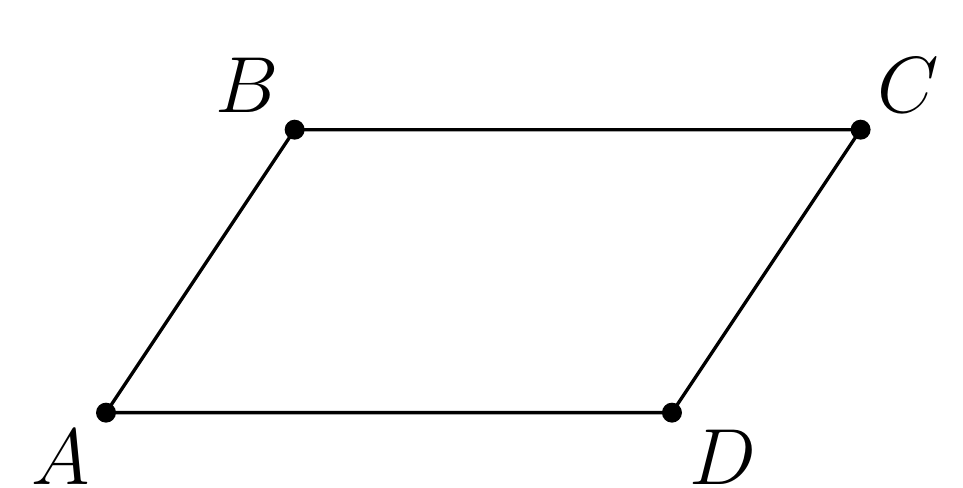
\includegraphics[scale = 0.3]{pic15.png}}
\end{figure}
\Solution По свойству у параллелограмма сумма градусных мер углов, прилежащих к одной стороне равна $180^{\circ}$. Значит больший угол параллелограмма равен 
\begin{center}$\dfrac{180^{\circ}+48^{\circ}}{2}=114^{\circ}$
\end{center}
\Answer{$114^{\circ}$}

